\pagestyle{empty}
\cleardoublepage
\pagestyle{fancy}

%Passos da modelagem:
%
%\begin{enumerate}[a.]
%	\item modelagem eletromagnética da parte passiva $\rightarrow$ Força passiva dependente de x,y,z
%	\item modelagem eletromagnética da parte ativa  $\rightarrow$ Força ativa de pedente de x,y,z,i
%	\item fundir modelos
%	\item modelagem da dinâmica e acoplamentos 
%\end{enumerate}

%Dimensões do mancal (Fig. \ref{Fig:Modelagem:Dimensoes})



%%--------------------------------------------
\chapter{Estator Interno}
%

O desenvolvimento do circuito ativo visa obter um atuador capaz de agir sobre o rotor fazendo com o que o mesmo mantenha-se em sua posição de equilíbrio ($d_x = 0 \, ; d_z = 0$) a través de forças geradas por campos eletromagnéticos via oito diferentes núcleos.

Cada núcleo age em colaboração com os núcleos vizinhos, sendo quatro núcleos principais e quatro secundários. Os núcleos principais estão localizados nos eixos radias do mancal (x,z), os núcleos secundários estão posicionados a uma distância angular de $45 ^\circ$. Essa topologia permite a maximização do fluxo magnético no eixo de interesse.

A parte ativa tem que ser capaz de vencer a força de atração gerada pelo circuito ativo quando o rotor estiver em sua excursão máxima. Para isso, criou-se um modelo analítico que representa essa parte do mancal e uma otimização numérica foi realizada visando a obtenção de um atuador dentro das especificações.

\begin{figure}[!ht]
	\centering
	\def\svgwidth{1\columnwidth}
	\includesvg{modelo_dim_ativo}
	\caption{Dimensões do mancal}
	\label{Fig:modelagem:dim:ativo}
\end{figure}

\section{Modelagem Magnética}

Parte da premissa que todas as linhas de campo magnético estão contidas nos componentes listados anteriormente e que o rotor encontra-se em sua posição de equilíbrio axial ($d_y = 0$) e sem inclinação. Considera-se o acionamento nas bobinas com uma tensão contínua e considerando o campo magnético estático.

\subsection{Campo Magnético no Entreferro}

A modelagem da parte ativa (atuadores) é realizada considerando o circuito magnético da Fig. \ref{Fig:modelagem:ativo:circuito2}, onde : $\mathcal{F}$ é a força contra eletromotriz gerada pela bobina; $R_n$ a relutância magnética associada ao núcleo da bobina; $R_g$ a relutância do entreferro; $R_r$ a relutância entre dois núcleos pelo ferro do rotor e $R_f$ a relutância de conexão entre dois núcleos pelo ferro de retorno do atuador.

\begin{figure}[h!]
	
		\begin{circuitikz}
			\draw (0,0)
	    	to[V,v^=$\mathcal{F}_1$] (0,2) 
			to[R=$R_{n1}$] (0,4) 
			to[R=$R_{gi1}$, i>^ =$\phi_1$] (0,6) 
			to[R=$R_{ri1}$] (2,6) 
			to[R=$R_{gi2}$,i=$\phi_2$] (2,4) 
			to[R=$R_{n2}$] (2,2) 
	    	to[V,v^=$\mathcal{F}_2$] (2,0) 
			to[R=$R_{fi1}$] (0,0); 			
			\foreach \i in {1,...,6}
			{
				\pgfmathtruncatemacro{\cur}{\i *2 + 2}
			    \pgfmathtruncatemacro{\pre}{\i *2 }
  			    \pgfmathtruncatemacro{\name}{\i+2}
  			     \pgfmathtruncatemacro{\namea}{\i+1}
					\draw (\pre,6)
					to[R=$R_{ri\namea}$] (\cur,6) 
					to[R=$R_{n\name}$] (\cur,4) 
					to[R=$R_{gi\name}$] (\cur,2) 
					to[V,v=$\mathcal{F}_\name$] (\cur,0)
					to[R=$R_{fi\namea}$] (\pre,0); 			
			}
			\draw (14,6)
			to[short](14,8)
			to[R=$R_{r8}$](0,8)
			to[short](0,6);
			\draw (14,0)
			to[short](14,-2)
			to[R=$R_{f8}$](0,-2)
			to[short](0,0);
		\end{circuitikz}


	\caption{Circuito magnético do circuito ativo}		\label{Fig:modelagem:ativo:circuito2}
\end{figure}

O desenvolvimento da modelagem foi realizado via análise de malhas. Adotando correntes internas no mesmo sentido, à cada malha pode-se escrever a seguinte equação geral:

\begin{align}
	(\sum R_m  - \sum  R_a ) \, \phi_m = \sum F_{EM} - \sum F_{CEM}
\end{align}

Sendo $\sum R_m$ e $I_m$  respectivamente a relutância e corrente interna de cada malha; $R_a$ e $I_{a}$ a relutância e corrente adjacente da malha e $F_{EM}$ a força contra eletromotriz positiva (sentido horário) e $\sum F_{CEM}$ a negativa. Obtemos as matrizes que representam o circuito:

\begin{align}
	\phi_m = 
	\begin{bmatrix}
	\phi_1 \\ \phi_2 \\  \phi_3 \\  \phi_4 \\  \phi_5 \\  \phi_6 \\  \phi_7 \\  \phi_8
	\end{bmatrix}
\end{align}

 \begin{align}
  R_m  = 
	\begin{bmatrix}
			 R_{m1} & 0 & 0 & 0 & 0 & 0 & 0 & 0 \\
			 0 & R_{m2} & 0 & 0 & 0 & 0 & 0 & 0 \\
			 0 & 0 & R_{m3} & 0 & 0 & 0 & 0 & 0 \\
			 0 & 0 & 0 & R_{m4} & 0 & 0 & 0 & 0 \\
			 0 & 0 & 0 & 0 & R_{m5} & 0 & 0 & 0 \\
			 0 & 0 & 0 & 0 & 0 & R_{m6} & 0 & 0 \\
			 0 & 0 & 0 & 0 & 0 & 0 & R_{m7} & 0  \\
 			 0 & 0 & 0 & 0 & 0 & 0 & 0 & R_{m8} 
	\end{bmatrix}
 \end{align}
 
Com:
 
 \begin{align}
	 R_{m1} &= R_{f1} + R_{n1} + R_{g1} + R_{r1} + R_{g2} + R_{n2} \\
	 R_{m2} &= R_{f2} + R_{n2} + R_{g2} + R_{r2} + R_{g3} + R_{n3}  \\
	 & \ldots \\
 	 R_{m3} &= R_{f8} + R_{n8} + R_{g8} + R_{r8} + R_{g1} + R_{n1}  \\
 \end{align}

E o componente devido a relutância adjacentes:

\begin{align}
R_a =
	\begin{bmatrix}
		R_{a1} \\ 	R_{a2} \\ 	R_{a3} \\ 	R_{a4} \\ 
		R_{a5} \\ 	R_{a6} \\ 	R_{a7} \\ 	R_{a8} 
	\end{bmatrix}
\end{align}

Sendo as relutância adjacente calculada como :

 \begin{align}
	 R_{a1} =& 
	 \begin{bmatrix}
			0 & R_{g2} + R_{n2} & 0 & 0 & 0 & 0 & 0 & R_{g8}+R_{n8}
	 \end{bmatrix} \\
	 R_{a2} =&
	 \begin{bmatrix}
		R{g1}+R{n1} & 0 & R{g3}+R_{n3} & 0 & 0 & 0 & 0 & 0
	 \end{bmatrix} \\
	 & \ldots \\
	 R_{a8} =&
	 \begin{bmatrix}
		R_{g1}+R_{n1} & 0 & 0 & 0 & 0  &0 & R_{g7}+R_{n7} & 0 
	 \end{bmatrix} 
 \end{align}

A matriz que correlaciona as forças contra eletromotriz :

\begin{align}
F_m = 
\begin{bmatrix}
	F_1 - F_2 \\
	F_2 - F_3 \\
	F_3 - F_4 \\
	F_4 - F_5 \\
	F_5 - F_6 \\
	F_6 - F_7 \\
	F_7 - F_8 \\
	F_8 - F_1 \\
\end{bmatrix}
\end{align}

Podemos resolver a equação do circuito com : $ \phi_m = (R_m - R_a) \, F_m^{-1}$, dado o resultado de cada fluxo eletromagnético nas malhas, é possível calcular os fluxos individuais nos entreferro ($\phi_g$). Uma vez encontrado o fluxo magnético, pode-se obter o campo magnético através da simples relação que engloba o fluxo e a área em que ele está distribuído.

\begin{align}
	\phi_g = 
	\begin{bmatrix}
		 \phi_1 - \phi_8 \\
		-\phi_1 + \phi_2 \\ 
		\phi_3 - \phi_2 \\ 
		-\phi_3 + \phi_4 \\ 
		\phi_5 - \phi_4 \\ 
		-\phi_5 + \phi_6 \\ 
		\phi_7- \phi_6  \\
		-\phi_7+ \phi_8 \\
	\end{bmatrix}
	\label{eq:ativo:fluxo:entreferro}
\end{align}

As relutâncias são calculadas utilizando as dimensões dos componentes do mancal com os comprimentos das linhas de campo ilustrado na Fig. \ref{Fig:modelagem:dim:ativo}. Resultando nas equações :

\begin{align}
R_{r}  &= \frac{l_r}{\mu_r \, S_r}			\\
R_{n} &= \frac{w_{n}}{\mu_{n}\, S_{n}}  \\     
R_{g} &= \frac{w_{gni}}{\mu_{0}\, S_{gni}}   \\    
R_{f} &= \frac{h_{fei}}{\mu_{f} \, S_{wfei}}    
\end{align}



\section{Forças}

A força resultante de atração referente  a cada bobina pode ser calculado pelo campo magnético acumulado no entreferro:

\begin{align}
	\vec{F_{nx}} = \frac{\vec{B}_{gx}^2 \; S_{gx}}{2 \mu_0} 
\end{align}

A força resultante projeta puramente no eixo normal ao núcleo principal é composto pela somatória das forças geradas pelos núcleos secundários, como mostrado na Fig. \ref{Fig:modelo:circuito:ativo:forcas}. Adotando que para pequenos deslocamentos no plano radial (x e y) a variação dos ângulos $\theta$ possam ser desprezíveis, obtemos:

\begin{align}
\vec{F}_y &= \vec{F}_{gn} + \cos(45) (\vec{F}_{ga} + \vec{F}_{gb}) \label{eq:ativo:F:resultante:y} \\
\vec{F}_x &= \cos(45) (\vec{F}_{ga} - \vec{F}_{gb})  \label{eq:ativo:F:resultante:x}
\end{align}

\begin{figure}[!ht]
	\centering
	\def\svgwidth{0.8\columnwidth}
	\includesvg{modelo_circuito_ativo_forcas}
		\caption{Forças resultante no rotor no eixo y}
		\label{Fig:modelo:circuito:ativo:forcas}
\end{figure} 


\section{Indutância} \label{subsec:at:indutancia}

O cálculo da indutância é importante pois atrela uma dinâmica ao atuador, a indutância está correlacionada a capacidade de geração de fluxo magnético de uma bobina e de sua corrente: $L = \frac {d\phi}{di}$. Das equações de densidade de campo magnético no entreferro de cada bobina:  Eq. \eqref{eq:ativo:fluxo:entreferro} encontra-se o fluxo magnético em cada núcleo.

Definindo o fluxo concentrado da bobina como o numero de espiras N pelo fluxo que a atravessa; A indutância própria com o  fluxo concentrado dividido pela corrente aplicada a bobina obtemos desconsiderando as demais fontes geradoras de fluxo, a indutância ($L$) em cada polo:

\begin{align}
	L_{a} &= \frac{\Phi_{fa}}{Ia} = N B_{ga}\biggr\rvert_{(I_b = 0, I_n = 0)} S_{ga} ,\ I_a^{-1} \\
	L_{b} &= \frac{\Phi_{fa}}{Ib} = N B_{gb}\biggr\rvert_{(I_a = 0, I_n = 0)} S_{gb} \, I_b^{-1} \\
	L_{n} &= \frac{\Phi_{fa}}{In} = N B_{gn}\biggr\rvert_{(I_a = 0, I_b = 0)} S_{gn} \, I_n^{-1} % = N^2 \mu_0 \ S_gn \, \frac{ C_2 + C_3}{S_{gn} + C_1 \, (C_2 + C_3)}
\end{align}

As indutâncias mutuas ($M$) são calculadas como sendo o fluxo que atravessa a bobina produzidas por outras fontes :

\begin{align}
M_{ab} &= \frac{\Phi_{b \rightarrow a}}{Ib} = N B_{ga}\biggr\rvert_{(I_a = 0, I_n = 0)} S_{ga} ,\ I_b^{-1} \\
M_{an} &= \frac{\Phi_{a \rightarrow n}}{Ia} = N B_{ga}\biggr\rvert_{(I_b = 0, I_n = 0)} S_{ga} ,\ I_a^{-1} \\
M_{ba} &= \frac{\Phi_{a \rightarrow b}}{Ib} = N B_{ga}\biggr\rvert_{(I_b = 0, I_n = 0)} S_{ga} ,\ I_b^{-1} \\
M_{bn} &= \frac{\Phi_{a \rightarrow b}}{I} = N B_{ga}\biggr\rvert_{(I_b = 0, I_n = 0)} S_{ga} ,\ I_b^{-1} \\
\end{align}

\section{Convergência}

Devido ao modelo apresentar componentes não lineares dado a curva de magnetização dos componentes ferro magnético do circuito, utilizamos o método de Newton-Rapson assim como no circuito passivo. Em cada nova interação, calcula-se as novas permeabilidades para os componentes compostos pelos: ferros do rotor, ferro do núcleo, ferro do estator interno e então resolve-se a equação de malha obtendo um novo resultado.

\section{Validação do Modelo}

O modelo analítico obtido é validado com o modelo desenvolvido em elementos finitos de três dimensões.

Dois tipos de analises foram realizadas nos modelos, a primeira, estipulando uma dimensão fixa a parte ativa do mancal e variando a corrente nas bobinas e a posição do rotor. A segunda, mantendo a mesma corrente e posição do rotor, variou-se algumas dimensões geométricas a fim de validar a robustez do modelo para diferentes geometrias.

A comparação entre os modelos no caso da variação da corrente e do deslocamento do rotor para uma determinada geometria pode ser analisado na Fig. \ref{Fig:simulacoes:ativo:comparacao:dx:i}. As forças obtidas por ambos modelos apresentam perfil e grandeza similares, porém os modelos divergem ligeiramente quando a corrente é máxima.

Isso acontece devido a saturação do ferro e o início da dispersão do campo magnético, influenciando tanto no fator de espraiamento quanto nas linhas de campo. 

	\begin{figure}[!ht]
		\subfloat[t][Modelo analítico]{
			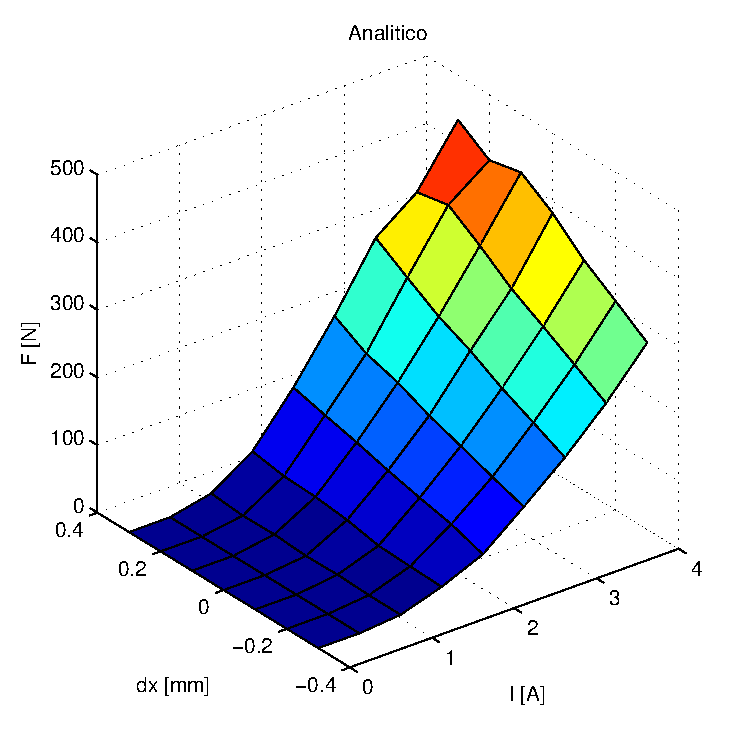
\includegraphics[width=0.5\linewidth]{Figs/Simulacoes/Ativo/validacao_ativo_map_analitico}
		}
		%
		\subfloat[b][Modelo em elementos finitos]{
		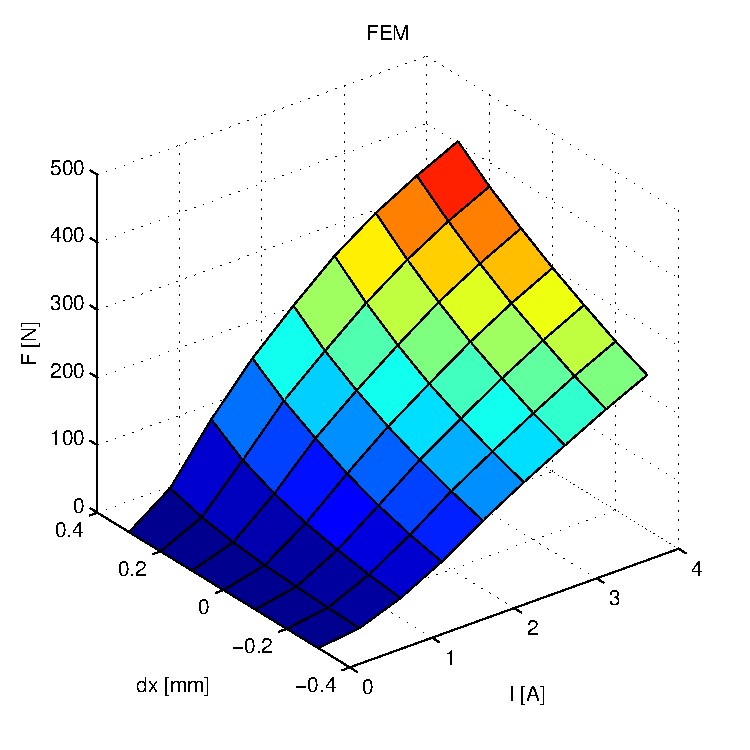
\includegraphics[width=0.5\linewidth]{Figs/Simulacoes/Ativo/validacao_ativo_map_fem}
		}	
		
		\caption{Modulo da força resultante devido o deslocamento do rotor e variação na corrente aplicada nas bobinas}
		\label{Fig:simulacoes:ativo:comparacao:dx:i}
	\end{figure}

A Fig. \ref{fig:validacao_ativo_2d} é um comparativo dos modelos quando submetidos a variação nos parâmetros construtivos, nesse caso variou-se a largura do núcleo da bobina ($w_n$), sua altura ($h_n$) e a largura do estator interno ($w_{fei}$). Nota-se a relação estreita entre os modelos quando as dimensões assumem valores maiores, a justificativa para tal fato é o desaparecimento de fluxos magnéticos não previstos no modelo analítico.

\begin{figure}[th]
	\centering
	\caption{Força magnética (N) x Variação de parâmetros}
	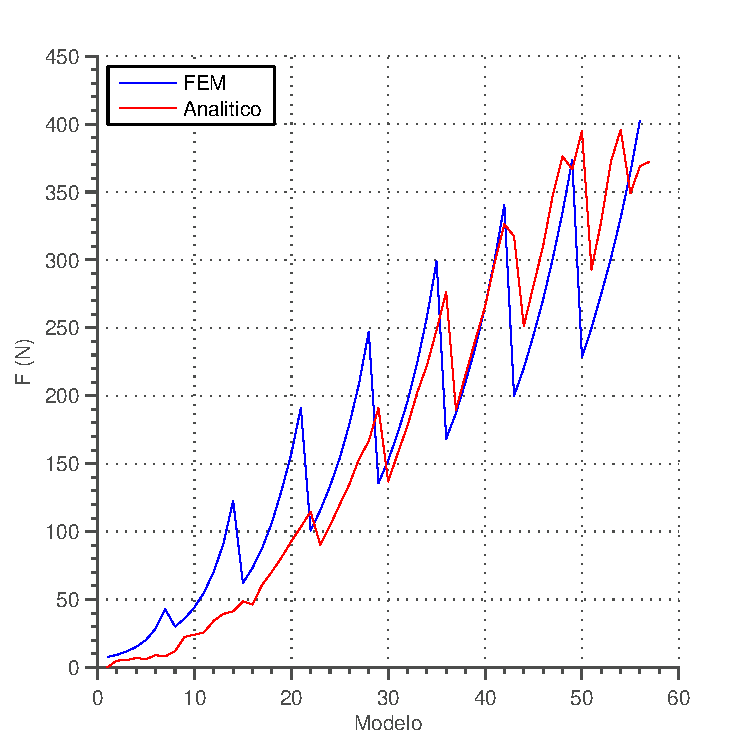
\includegraphics[width=0.7\linewidth]{Figs/Simulacoes/Ativo/validacao_ativo_2d}
	\caption{Comparativo entre modelos quanto a variação da geometria}
	\label{fig:validacao_ativo_2d}
\end{figure}

\section{Otimização dos Parâmetros}

Os parâmetros que devem ser otimizados são aqueles que não influenciam na topologia definida para a parte passiva do mancal, já que a mesma foi otimizada separadamente. Optou-se por não realizar uma otimização de ambas as partes simultaneamente evitando o problema da dimensionalidade.

As variáveis a serem otimizadas nesse etapa do projeto são: o entreferro interno ($g_{gi}$), o comprimento ($w_n$) altura  e largura ($l_n$) do núcleo da bobina ($h_n$) e a quantidade de espiras da bobina ($n_n$). O atuador tem que ser capaz de vencer a força de atração de 160N gerada pelo circuito passivo quando o rotor encontra-se no maior deslocamento (0.3 mm, limitado pelo batente). 

Uma ponto levado em consideração nessa etapa foi a da área útil para ser instalado as bobinas, esse espaço restrito é limitado pelo tamanho do ferro e pela largura do núcleo da bobina. A Fig. \ref{fig:modelo_ativo_bobina} ilustra a área em que a bobina é localizada. O cálculo essa área ($S_{bob}$) leva em consideração a secção do fio utilizado ($S_{fio}$), o fator de embobinamento ($K_b$) e a quantidade de voltas de espiras, podendo ser calculado como:

\begin{align}
	S_{bob} = 2 \, n_n \, \, S_{fio} \, K_b
\end{align}

Durante a otimização, verifica-se se a área útil para embobinamento é satisfeita, caso contrário, o modelo obtido é descartado e uma nova otimização é realizada.

\begin{figure}[ht!]
\centering
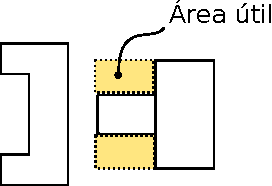
\includegraphics[width=0.7\linewidth]{Figs/modelo_ativo_bobina}
\caption{Área útil para embobinamento de cada núcleo}
\label{fig:modelo_ativo_bobina}
\end{figure}

Os parâmetros geométricos iniciais ($L_0$) do estator interno foram levantados partindo da restrição de potência imposta pela especificação da Tab. \ref{tab:PMM:especificações}, com a potência (100W) e  tensão elétrica de alimentação (24V) obtemos a corrente máxima de trabalho (4A). Essa corrente elétrica deve ser suficiente para gerar uma força de atração que consiga compensar a força gerada pelo circuito passivo no maior entreferro, levantada no modelo em elementos finitos (160N). Da equação de força magnética ($\nicefrac{B^2.A}{(l/\mu +2g)^2}$ ) foi possível encontrar uma aproximação da área do polo necessária para gerar uma força capaz de vencer a força imposta pelo ímã. Com um valor inicial da área transversal do polo, definiu-se o número de voltas das bobinas necessária para gerar o fluxo magnético no entreferro. Com a área útil e a quantidade de voltas definiu-se a bitola do filamento com resistência elétrica capaz de gerar a corrente de 4A (AWG 33).

A otimização foi realizada via método de Nelder-Mead Simplex com restrições, limitando assim a dimensão máxima do mancal e evitando que a topologia proposta sofra alterações ao longo das interações e que dimensões que ferem as especificações sejam obtidas. A condição inicial obtida do método lista anteriormente assim como as restrições são listas na Tab. \ref{tab:ativo:restrições}.

\begin{table}[ht!]
	\centering
	\begin{tabular}{c c c c c c c}
					 & $w_{gi}$ & $n_n$ & $h_n$ & $w_n$ &  $l_n$   \\ \hline \hline
		$L_{0}$  &  0.6 & 300  &   10 &  22 & 6  &   12 \\
		$L_{Min}$&  0.4 & 50   &   5  &  10 & 3  &   6	\\
		$L_{Max}$ & 1.2 & 600  &   20 &  30 & 10 &   22
	\end{tabular} 
	\caption{Valores iniciais, máximos e mínimos utilizado na otimização, valores em milímetros.}
	\label{tab:ativo:restrições} 
\end{table}

A função mérito utilizada no projeto do atuador engloba a força de atração $F_b$ resultante da aplicação de uma corrente de quatro Amperes no núcleo principal e de dois Amperes nos núcleos secundários, a indutância da bobina ($L_b$) e do volume do estator interno ($V_{ma}$). Busca-se um modelo que possua maior força de atração, baixa indutância e menor volume. Os pesos utilizados durante a otimização 

\begin{align}
	P_1 &= 3 \, 10^2/ F_b \\
	P_2 &= 15 \, 10^4 \, L_b \\
	P_3 &= 10^6 \, V_{ma} \\
	P_4 &= \frac{25 \, 10^{-4}}{w_{gi}}				\\
	F   &= P_1 + P_2 + P_3 + P_4
\end{align}

A evolução dos parâmetros ao longo da otimização é ilustrado na Fig. \ref{fig:otimizacao_ativo_parametros}. Durante a interação, verificamos o acréscimo da força de atração,  maior ponderação durante o processo de otimização.  A evolução do valor do entreferro assume um valor médio, já que seu valor influência diretamente na força de atração. A Fig. \ref{fig:otimizacao_ativo_pesos} demonstra a evolução dos pesos propostos para o funcional ao longo da otimização. Obtém com a otimização proposta um mancal com volume inferior do inicialmente proposto com indutância diminuída.

\begin{figure}[ht!]
	\centering
	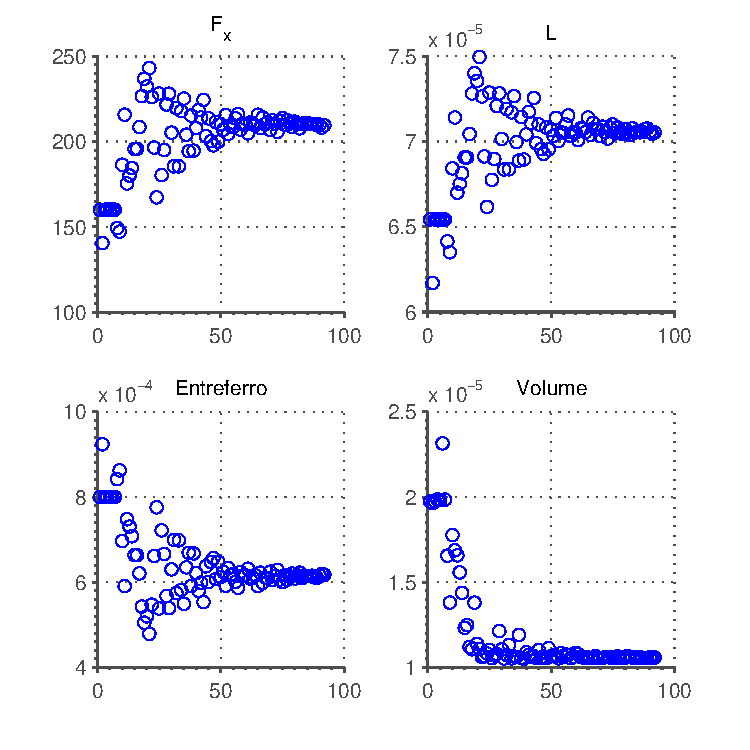
\includegraphics[width=0.6\linewidth]{Figs/Simulacoes/Ativo/otimizacao_ativo_parametros}
	\caption{Evolução dos parâmetros construtivos do mancal ao longo da otimização}
	\label{fig:otimizacao_ativo_parametros}
\end{figure}

\begin{figure}[ht!]
\centering
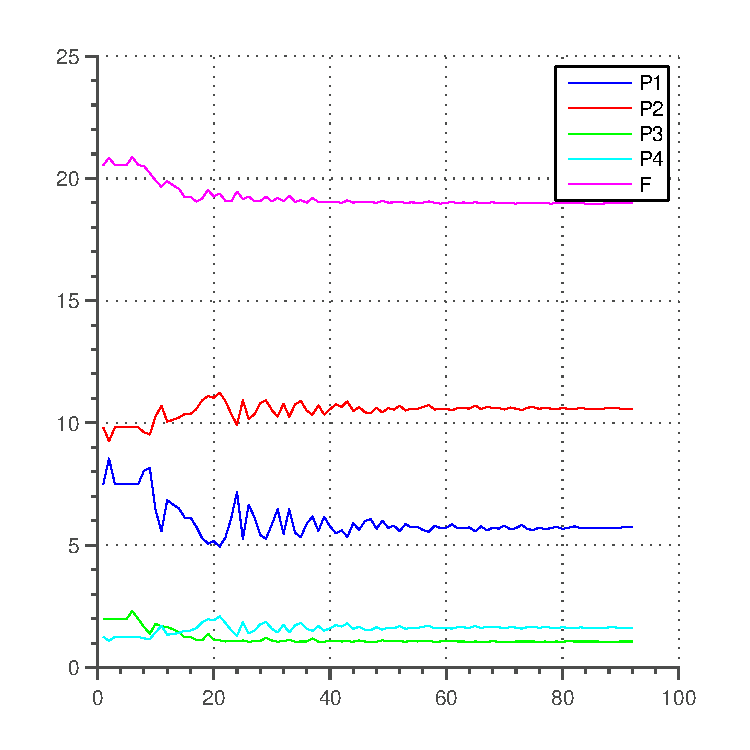
\includegraphics[width=0.6\linewidth]{Figs/Simulacoes/Ativo/otimizacao_ativo_pesos}
\caption{Evolução dos pesos propostos para o funcional ao longo da otimização}
\label{fig:otimizacao_ativo_pesos}
\end{figure}


\section{Mancal Ativo Resultante da Otimização}

O mancal ativo resultante possui dimensões listadas na Tab. \ref{tab:ativo:resultado}. A força de atração resultante da excitação das bobinas com uma corrente principal de quatro Amperes com o rotor no seu deslocamento máximo e sob o efeito da atração oposto do circuito passivo é de 23 N , ou seja, o atuador proposto é capaz de retirar o rotor de sua posição de máximo deslocamento e o mover para seu ponto de operação.

\begin{table}[ht!]
	\centering
	\begin{tabular}{c c c c c}
		 $w_{gi}$ 	& $n_n$ & $h_n$ & $w_n$ & $w_{fei}$  \\ \hline \hline
		 0.7		& 300  	& 10.8 	& 14.9	& 6
	\end{tabular} 
	\caption{Mancal ativo obtido devido a otimização, valores em milímetros}
	\label{tab:ativo:resultado} 
\end{table}

A curva de força ($F_b$) por deslocamento é ilustrado na Fig. \ref{ativo_otimizado_fem_I_dx03}, nessa simulação o rotor está deslocado de 0.3 milímetros de sua posição nominal, as bobinas exitadas são aquelas do mesmo sentido do deslocamento do rotor, gerando assim, uma força de atração oposta a do estator externo.  

\begin{figure}[ht!]
\centering
Força de atração (N) x Corrente (A)
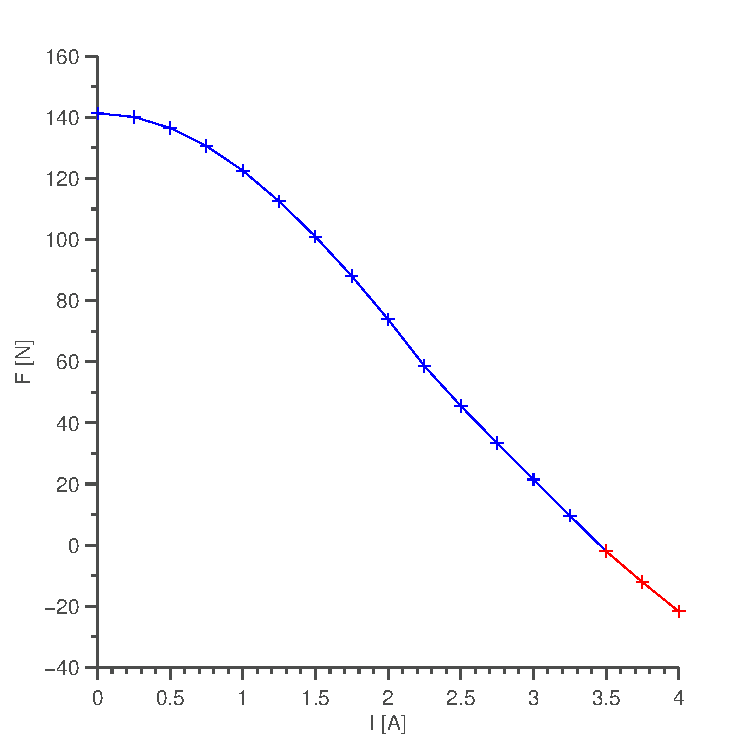
\includegraphics[width=0.8\linewidth]{Figs/Simulacoes/Ativo/ativo_otimizado_fem_I_dx03}
\caption{Força resultante da aplicação de uma corrente quando o rotor está deslocado de 0.3 mm (máxima distância)}
\label{ativo_otimizado_fem_I_dx03}
\end{figure}

Verifica-se que a força gerada pelas bobinas vence a força gerada pelo estator externo quando uma corrente superior á $3.5$ Ampères é aplicada no polo principal. A curva de força por corrente nesse ponto de operação é não linear, o que dificulta o projeto do controlador.

No caso da operação em torno do ponto de equilíbrio, a força atuante no rotor possui a forma da Fig. \ref{ativo_otimizado_fem_I_dx00}. Nessa situação, as forças de tração devido ao estator externa possui resultante nula, e a única força atuante no rotor é a da gerada pela corrente nos polos. Verfica-se que o delta de força nesse caso é de $220$ N contra $180$ N do rotor na excursão máxima, isso se da devido ao menor entreferro entre o polo e o rotor.

\begin{figure}[ht!]
\centering
Força de atração (N) x Corrente (A)
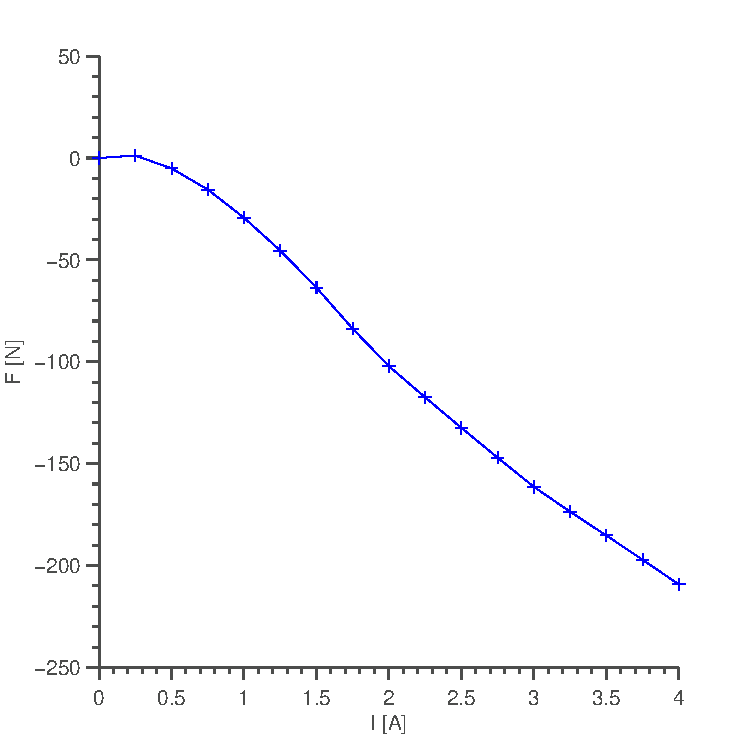
\includegraphics[width=0.8\linewidth]{Figs/Simulacoes/Ativo/ativo_otimizado_fem_I_dx00}
\caption{Força resultante da aplicação de uma corrente quando o rotor está em seu ponto de operação}
\label{ativo_otimizado_fem_I_dx00}
\end{figure}

O campo magnético no polo principal devido a variação na corrente elétrica é ilustrado na Fig. \ref{fig:ativo:fem:b:polos}, notasse os diferentes pontos de operação do componente magnético quando o rotor é mantido na mesma posição. Pela simulação é possível notar que o espraiamento da área sofre aumento com a corrente, dinâmica não levada em consideração na modelagem analítica. 

\begin{figure}[!ht]
	\centering
	\subfloat[a][I = 1 A]{
	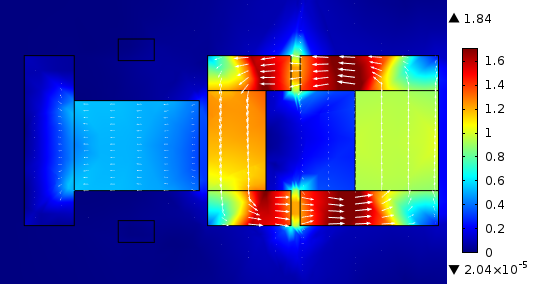
\includegraphics[width=0.4\linewidth]{Figs/Simulacoes/Ativo/dx=03_I=1}
	}
	\subfloat[b][I = 2 A]{
	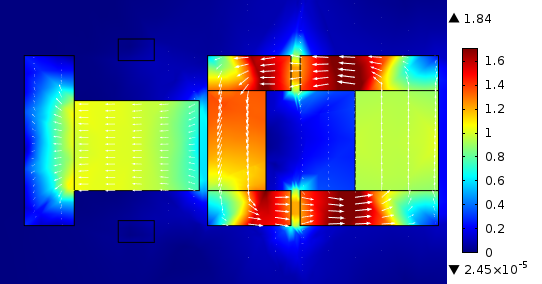
\includegraphics[width=0.4\linewidth]{Figs/Simulacoes/Ativo/dx=03_I=2}
	}	\\
	\subfloat[c][I = 3 A]{
	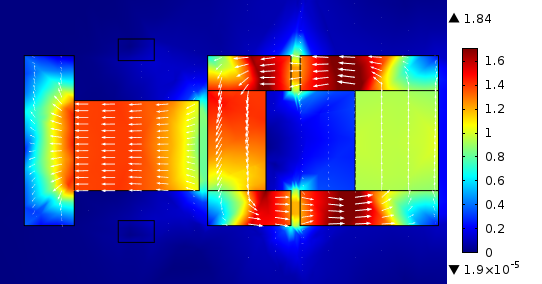
\includegraphics[width=0.4\linewidth]{Figs/Simulacoes/Ativo/dx=03_I=3}
	}
	\subfloat[d][I = 4 A]{
	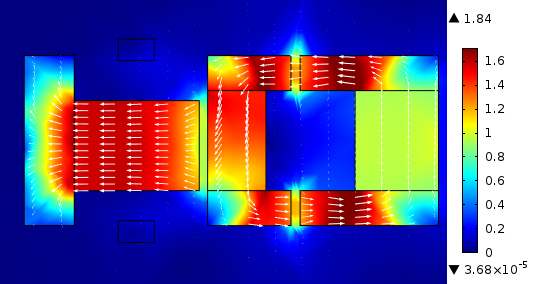
\includegraphics[width=0.4\linewidth]{Figs/Simulacoes/Ativo/dx=03_I=4}
	}	
	\caption{Vetor campo magnético no polo principal quando variado a corrente, rotor com deslocamento de 0.3mm de sua posição.}
	\label{fig:ativo:fem:b:polos}
\end{figure}

Através de um corte axial verificamos que as linhas de campo magnético são contidas nos polos ativos, isso ocorre devido a polarização das correntes nos polos secundários, forçando o fluxo por eles. Verificamos também que o componente magnético responsável pela maior contribuição na relutância é o núcleo da bobina principal (polo).

\begin{figure}
\centering
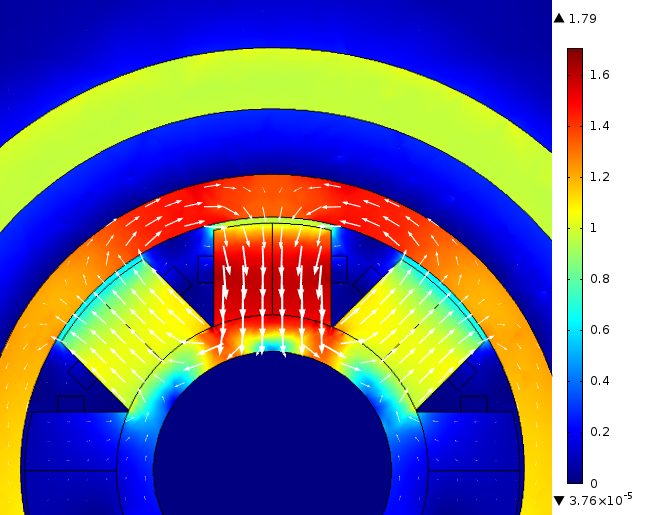
\includegraphics[width=0.8\linewidth]{Figs/Simulacoes/Ativo/Cima_dx=03_I=4}
\caption{Vetor campo magnético de uma secção radial do mancal quando aplicado uma corrente de 4A no polo principal}
\label{fig:ativo:fem:b:radial}
\end{figure}




